\documentclass[aspectratio=169]{beamer}

\usepackage[utf8]{inputenc}
\usepackage[english]{babel}
\usepackage{lmodern}
\usepackage{amsmath}
\usepackage{amsfonts}
\usepackage{amssymb}
\usepackage{graphicx}
\usepackage{booktabs}
\usepackage{xcolor}
\usepackage{tikz}
\usepackage{pgf}
\def\mathdefault#1{#1}
\usepackage{algorithm}
\usepackage{algpseudocode}

% Font configuration for PGF compatibility
\usepackage{ifxetex,ifluatex}
\newif\ifxetexorluatex
\ifxetex
  \xetexorluatextrue
\else
  \ifluatex
    \xetexorluatextrue
  \else
    \xetexorluatexfalse
  \fi
\fi

\ifxetexorluatex
  \usepackage{fontspec}
  \setmainfont{EB Garamond}
  \setmonofont[Scale=MatchLowercase]{Source Code Pro}
\else
  \usepackage[lf]{ebgaramond}
  \usepackage[oldstyle,scale=0.7]{sourcecodepro}
\fi

% Theme
\usetheme{Madrid}
\usecolortheme{default}

% Title page information
\title[Multi-Dataset Training for Image Classification]{Research and Implementation of Multi-Dataset Training for Image Classification with Discrepant Taxonomies}
\subtitle{Master Thesis Presentation}
\author{Björn Buschkämper}
\institute[Bielefeld University]{Technical Faculty, Bielefeld University}
\date{September 19, 2025}

\begin{document}

% Title slide
\begin{frame}
    \titlepage
\end{frame}

% Outline
\begin{frame}{Outline}
    \tableofcontents
\end{frame}

% Section 1: Introduction & Motivation
\section{Introduction \& Motivation}

\begin{frame}{The Challenge: Limited Scope of Traditional Models}
    \begin{itemize}
        \item Traditional image classification models are trained on specific datasets
        \item Each model recognizes only a predefined set of categories
        \item Multiple models needed for different domains = inefficient storage and deployment
    \end{itemize}

    \vspace{1em}

    \textbf{Current Approaches:}
    \begin{itemize}
        \item \textbf{Transfer Learning}: Adapt pre-trained models to new tasks
        \item \textbf{Multi-head Architecture}: Shared backbone + task-specific heads
    \end{itemize}

    \vspace{1em}

    \textcolor{red}{\textbf{Problem:}} Still requires separate models or heads for each domain
\end{frame}

\begin{frame}{Our Idea: Universal Model vs. Multi-Head}
    \begin{columns}[T]
        \begin{column}{0.48\textwidth}
            \textbf{Multi-Head Approach}
            \begin{itemize}
                \item Shared backbone
                \item Task-specific heads
                \item Automatic feature distillation
                \item Domain alignment challenges
            \end{itemize}

            \begin{center}
                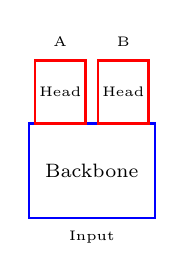
\begin{tikzpicture}[scale=0.8]
                    % Backbone
                    \draw[thick, blue] (0,0) rectangle (2,1.5);
                    \node at (1,0.75) {\scriptsize Backbone};

                    % Heads (made wider)
                    \draw[thick, red] (0.1,1.5) rectangle (0.9,2.5);
                    \node at (0.5,2) {\tiny Head};
                    \draw[thick, red] (1.1,1.5) rectangle (1.9,2.5);
                    \node at (1.5,2) {\tiny Head};

                    % Labels
                    \node at (1,-0.3) {\tiny Input};
                    \node at (0.5,2.8) {\tiny A};
                    \node at (1.5,2.8) {\tiny B};
                \end{tikzpicture}
            \end{center}
        \end{column}

        \begin{column}{0.48\textwidth}
            \textbf{Universal Model Approach}
            \begin{itemize}
                \item Single shared model
                \item Universal output layer
                \item Predefined concept mapping
                \item Static domain conversion
            \end{itemize}

            \begin{center}
                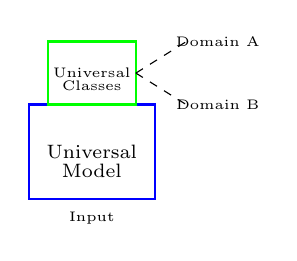
\begin{tikzpicture}[scale=0.8]
                    % Model
                    \draw[thick, blue] (0,0) rectangle (2,1.5);
                    \node at (1,0.75) {\scriptsize Universal};
                    \node at (1,0.45) {\scriptsize Model};

                    % Universal output (made wider)
                    \draw[thick, green] (0.3,1.5) rectangle (1.7,2.5);
                    \node at (1,2) {\tiny Universal};
                    \node at (1,1.8) {\tiny Classes};

                    % Conversion
                    \draw[dashed] (1.7,2) -- (2.5,2.5);
                    \draw[dashed] (1.7,2) -- (2.5,1.5);
                    \node at (3,2.5) {\tiny Domain A};
                    \node at (3,1.5) {\tiny Domain B};

                    % Labels
                    \node at (1,-0.3) {\tiny Input};
                \end{tikzpicture}
            \end{center}
        \end{column}
    \end{columns}

    \vspace{1em}

    \textcolor{blue}{\textbf{Our task:}} Discover inter-dataset class relationships to build a universal taxonomy
\end{frame}

\begin{frame}{Our Method in 3 Steps}
    \begin{center}
        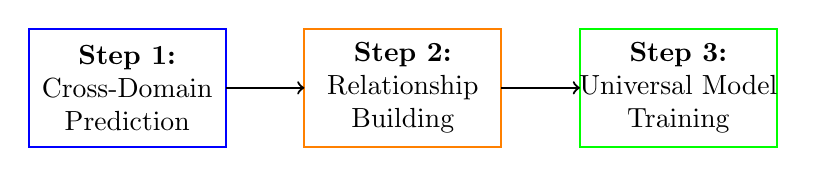
\begin{tikzpicture}[node distance=3cm]
            % Step 1
            \draw[thick, blue] (0,0) rectangle (2.5,1.5);
            \node[align=center] at (1.25,0.75) {\textbf{Step 1:}\\Cross-Domain\\Prediction};

            % Step 2
            \draw[thick, orange] (3.5,0) rectangle (6,1.5);
            \node[align=center] at (4.75,0.75) {\textbf{Step 2:}\\Relationship\\Building};

            % Step 3
            \draw[thick, green] (7,0) rectangle (9.5,1.5);
            \node[align=center] at (8.25,0.75) {\textbf{Step 3:}\\Universal Model\\Training};

            % Arrows
            \draw[->, thick] (2.5,0.75) -- (3.5,0.75);
            \draw[->, thick] (6,0.75) -- (7,0.75);
        \end{tikzpicture}
    \end{center}

    \vspace{1em}

    \begin{enumerate}
        \item \textbf{Cross-Domain Prediction}: Train domain-specific models, run inference on other domains
        \item \textbf{Relationship Building}: Extract meaningful relationships from cross-domain predictions and create universal taxonomy
        \item \textbf{Universal Model Training}: Create and train a single model using universal taxonomy
    \end{enumerate}
\end{frame}

\begin{frame}{Changes to Method of Bevandic et al.}
    \begin{enumerate}
        \item \textbf{Weighted Relationships:} Instead of binary, unweighted relationships, we use weighted relationships to capture the strength of associations between classes.
        \item \textbf{Relationship Selection Methods:} We try multiple methods to select the most relevant relationships from noisy cross-domain predictions.
        \item \textbf{Discrete Probability Loss Function:} We use a loss function that allows training with probability distributions as targets, enabling the model to learn from the uncertainty in class relationships.
        \item \textbf{Adapted to Image Classification:} The original method was designed for image segmentation, we adapt it for image classification tasks.
    \end{enumerate}
\end{frame}

% Section 2: Method Overview
\section{Method Overview}

\begin{frame}{Cross-Domain Prediction Process}
    \textbf{Goal}: Discover relationships between classes from different datasets

    \vspace{0.5em}

    \textbf{Process}:
    \begin{enumerate}
        \item Train domain-specific models
        \item Run each model on images from \emph{all other} domains, building prediction matrices $M_{ab}(i,j)$ = number of times class $c_i^a$ predicted as class $c_j^b$
        \item Create probability matrices $P_{ab}(i,j)$ = probability of classifying class $c_i^a$ as class $c_j^b$
    \end{enumerate}

    \vspace{0.5em}

    \begin{equation}
        P_{ab}(i, j) = \frac{M_{ab}(i, j)}{\sum_{k=1}^{|C_a|} M_{ab}(i, k)}
    \end{equation}

    \vspace{0.5em}

    \textbf{Example}: Caltech-256 class "car" predicated by CIFAR-100 model as "vehicle" ($80\%$), "bike" ($18\%$), "butterfly" ($2\%$)
\end{frame}

\begin{frame}{Challenge: Selecting Relevant Relationships}
    \textbf{Problems with raw probability matrices}:
    \begin{itemize}
        \item Noisy predictions from imperfect models
        \item Unknown number of true relationships
        \item Different datasets have different scales of similarity
    \end{itemize}

    \vspace{1em}

    \textbf{Solution}: Develop multiple relationship selection methods and compare their effectiveness
\end{frame}

\begin{frame}{Relationship Selection Methods Explained}
    \begin{enumerate}
        \item \textbf{Most Common Foreign Prediction (MCFP) by Bevandic et al.}:
              \begin{equation}
                  \text{select\_relationships}(P_{ab}) = \{(i, j) \mid j = \text{argmax}_{j'} P_{ab}(i, j')\}
              \end{equation}

        \item \textbf{Naive Thresholding}:
              \begin{equation}
                  \text{select\_relationships}(P_{ab}) = \{(i, j) \mid P_{ab}(i, j) \geq t\}
              \end{equation}

        \item \textbf{Density Thresholding}: Select minimum relationships covering $p\%$ of probability mass

        \item \textbf{Relationship Hypothesis}: Assumes relationships based on shared concepts should have equal probabilities. For each class, find optimal $k$ relationships by minimizing:
              \begin{equation}
                  \sum_{j=1}^k \left| X_i(j) - \frac{1}{k} \right| + \sum_{j=k+1}^{|C_b|} X_i(j)
              \end{equation}
              where $X_i(j)$ are sorted probabilities in descending order.
    \end{enumerate}
\end{frame}


% Section 4: Universal Model
\section{Universal Model}

\begin{frame}{Universal Taxonomy Building Rules}
    \textbf{How do we convert relationship graphs into universal taxonomies?}

    \vspace{0.5em}

    \begin{enumerate}
        \item \textbf{Isolated Node Rule}: Classes with no relationships
              \begin{itemize}
                  \item Create new universal class for standalone domain classes
                  \item Ensures all classes are represented in universal taxonomy
              \end{itemize}

        \item \textbf{Bidirectional Relationship Rule}: Classes with mutual relationships (A $\leftrightarrow$ B)
              \begin{itemize}
                  \item Create single universal class C with relationships A $\rightarrow$ C, B $\rightarrow$ C
                  \item Indicates classes likely represent the same concept
              \end{itemize}

        \item \textbf{Transitive Cycle Rule}: Prevent invalid cycles (A $\rightarrow$ B $\rightarrow$ C where A, C same domain)
              \begin{itemize}
                  \item Remove relationship with lower probability
                  \item Classes within same domain should be disjoint
              \end{itemize}

        \item \textbf{Unilateral Relationship Rule}: Handle subset relationships (A $\rightarrow$ B)
              \begin{itemize}
                  \item Create universal class for shared concepts (A $\cup$ B)
                  \item Create universal class for unique concepts (B only)
              \end{itemize}
    \end{enumerate}
\end{frame}

\begin{frame}{Taxonomy Visualization (Caltech-101 + Caltech-256)}
    \begin{center}
        \includegraphics[width=0.5\textwidth]{../thesis/figures/taxonomy.png}
    \end{center}
\end{frame}

\begin{frame}{Good Cluster}
    \begin{center}
        \includegraphics[width=0.35\textwidth]{../thesis/figures/wheel_concept.png}
    \end{center}
\end{frame}

\begin{frame}{Bad Cluster}
    \begin{center}
        \includegraphics[width=0.5\textwidth]{../thesis/figures/bad_taxonomy.png}
    \end{center}
\end{frame}

\begin{frame}{Building the Universal Model}

    \begin{itemize}
        \item Every universal class corresponds to one output neuron
        \item Each domain class maps to one or more universal classes
        \item Matrix $M_i$ maps domain $i$ classes to universal classes
    \end{itemize}

    \vspace{1em}

    \textbf{Target Generation}: Convert domain labels to universal class distributions
    \begin{equation}
        \mathbf{t} = \hat{M}_i[j, :] \quad \text{where } \hat{M}_i(j, u) = \frac{M_i(j, u)}{\sum_{u'} M_i(j, u')}
    \end{equation}

    \textbf{Loss Function}:
    \begin{equation}
        \mathcal{L} = -\sum_{u=1}^{|U|} \mathbf{t}(u) \log(\mathbf{p}(u))
    \end{equation}
\end{frame}

\begin{frame}{Multi-Domain Training Process}
    \textbf{Training Procedure}:
    \begin{enumerate}
        \item Concatenate domain datasets
        \item Each sample: $(\text{image}, (\text{domain\_id}, \text{label})) \rightarrow (\text{image}, \text{universal\_target})$
        \item Train universal model on unified dataset
    \end{enumerate}

    \vspace{1em}

    \textbf{Inference}:
    \begin{align}
        \mathbf{d}_i & = M_i^T \mathbf{p}            \\
        \hat{c}_i    & = \text{argmax}(\mathbf{d}_i)
    \end{align}

    where $\mathbf{p}$ are universal class predictions and $\hat{c}_i$ is the predicted class in domain $i$.
\end{frame}

% Section 5: Results
\section{Results}

\begin{frame}{Universal Model Performance}
    \textbf{Datasets}: Caltech-101, Caltech-256, CIFAR-100

    \begin{columns}[T]
        \begin{column}{0.48\textwidth}
            \textbf{Cal-101 + Cal-256 Results}
            \begin{table}[h]
                \centering
                \tiny
                \begin{tabular}{lcc}
                    \toprule
                    \textbf{Taxonomy} & \textbf{Cal-101}       & \textbf{Cal-256}        \\
                    \midrule
                    Hypothesis        & 91.81 (+0.00)          & 82.84 (+13.36)          \\
                    MCFP              & 91.23 (-0.58)          & 80.75 (+11.27)          \\
                    MCFP Binary       & 92.73 (+0.92)          & \textbf{89.71 (+20.23)} \\
                    Density           & 92.96 (+1.15)          & 81.54 (+12.06)          \\
                    Naive             & \textbf{93.19 (+1.38)} & 82.25 (+12.77)          \\
                    \bottomrule
                \end{tabular}
            \end{table}
        \end{column}

        \begin{column}{0.48\textwidth}
            \textbf{Cal-101 + Cal-256 + CIFAR Results}
            \begin{table}[h]
                \centering
                \tiny
                \begin{tabular}{lccc}
                    \toprule
                    \textbf{Taxonomy} & \textbf{Cal-101}       & \textbf{Cal-256}        & \textbf{CIFAR}          \\
                    \midrule
                    Hypothesis        & 68.74 (-23.07)         & 58.17 (-11.31)          & 69.03 (+8.55)           \\
                    MCFP              & 83.28 (-8.53)          & 76.50 (+7.02)           & 76.10 (+15.62)          \\
                    MCFP Binary       & 94.58 (+2.77)          & 85.13 (+15.65)          & 82.71 (+22.23)          \\
                    Density           & 95.39 (+3.58)          & 83.53 (+14.05)          & \textbf{83.14 (+22.66)} \\
                    Naive             & \textbf{95.50 (+3.69)} & \textbf{85.36 (+15.88)} & 72.56 (+12.08)          \\
                    \bottomrule
                \end{tabular}
            \end{table}
        \end{column}
    \end{columns}

    \vspace{0.5em}

    \textbf{Baselines}: Cal-101: 91.81\%, Cal-256: 69.48\%, CIFAR-100: 60.48\%

    \textbf{Key Findings}:
    \begin{itemize}
        \item Universal models \textcolor{blue}{\textbf{outperform}} single-domain baselines
        \item Different relationship selection methods excel on different datasets
    \end{itemize}
\end{frame}

% Section 6: Conclusion
\section{Conclusion}

\begin{frame}{Key Contributions}
    \begin{enumerate}
        \item \textbf{Novel Weighted Graph Approach}: We have a \textit{weighted} relationship graph instead of binary edges

        \item \textbf{Comprehensive Relationship Selection Methods}: Four different methods to select relevant relationships from noisy predictions

        \item \textbf{Reusable Taxonomy Framework}: Our code is adaptable to new taxonomy building rules,
              relationship selection methods, datasets and model architectures

        \item \textbf{Full-automatic, multi-dataset training pipeline}: We provide a complete pipeline for training on multiple datasets without manual intervention or preprocessing
    \end{enumerate}
\end{frame}

\begin{frame}{Future Work}
    \textbf{Findings}:
    \begin{itemize}
        \item Bad clusters still exist in universal taxonomies
        \item Multi-domain universal model training outperforms single-domain training
        \item No single relationship selection method is best for all cases
    \end{itemize}

    \vspace{1em}

    \textbf{Future Work}:
    \begin{itemize}
        \item Adaptive or hybrid relationship selection method to get best performance
        \item Extended tests on larger, more diverse taxonomies and datasets
        \item Application to other tasks (e.g., object detection, image segmentation)
    \end{itemize}
\end{frame}

\begin{frame}{Questions?}
    \begin{center}
        \textbf{\Large Thank you for your attention!}

        \vspace{1em}

        \textbf{Questions?}
    \end{center}
\end{frame}

\end{document}